\section{Minimum spanning trees}

In a connected graph, a spanning tree is a tree that contains all nodes
and a subset of the edges.
A minimum spanning tree is a spanning tree with minimum total length.
An example is given below:
\begin{center}
    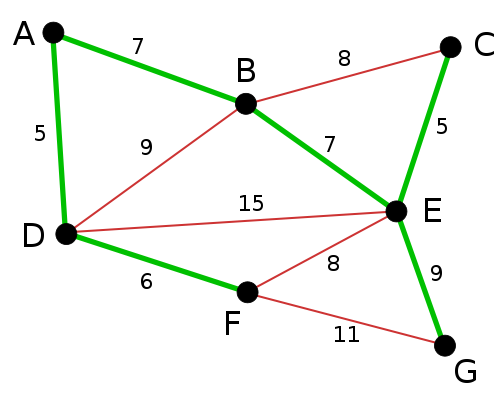
\includegraphics[width=0.3\textwidth]{img/spanning}
\end{center}

Finding the minimum spanning tree means finding the shortest edges in total
that keep the graph connected.

\subsection{Kruskal's algorithm}

In order to construct the minimum spanning tree, Kruskal's algorithm
just picks the smallest edges first, unless adding them forms a cycle
(it would not be a tree anymore).
This is a greedy approach, and surpisingly it works.

To check if adding an edge, we can check if they belong to the same
connected component.
Since those connected components are merged together as we add edges,
they will best be represented with a union-find data structure.

The algorithm goes through the edges in increasing order of weight.
For each edge $(u,v)$, if $u$ and $v$ are in different components,
add $(u,v)$ to the tree and unite their components;
otherwise, discard the edge.

The complexity is $O(m \log m)$.

\subsection{Prim's algorithm}

The approach of Prim's algorithm is slightly different from Kruskal's.
Instead of looking at the shortest edges in the whole graph,
it begins with a starting point and picks edges to add around it.
That way it will slowly spread to the whole graph,
each time choosing the shortest edge that is in contact with the current zone.

It traverses the graph in nearly the same way as Dijkstra's algorithm,
the only difference being that Dijstra picks vertices according to their total
distance from the starting point, while for Prim only the last edge matters.
Usually, only one line needs to be changed.

When implemented with a heap, Prim's complexity is also
$O(m\log m)$.

